% !TeX root = surprises.tex

\selectlanguage{hebrew}

\chapter{מחוגה מתמוטטת}\label{c.collapse}

%%%%%%%%%%%%%%%%%%%%%%%%%%%%%%%%%%%%%%%%%%%%%%%%%%%%%%%%%%%%%%%

במחוגה מודרנית היא 
\textbf{מחוגה קבועה}:
ניתן לקבע את המרחק בין שתי הרגליים וכך להעתיק קטע קו או מעגל ממקום למקום (%
\ref{fig.fixed-compass}).
אוקלידס השתמש במחוגה 
\textbf{מתמוטטת}
\L{(collapsing)}
בה לא ניתן לשמור מרחק קבוע (%
\ref{fig.collapsing-compass}).
שרגליה מתקפלות כאשר מרימים אותן מהנייר. לעתים קרובות מורים משתמשים מחוגה מתמוטטת המורכבת מטוש שמחובר לחוט כדי לבנות מעגל הלוח. אי-אפשר לשמור על מרחק קבוע כאשר מרימים את המחוגה מהלוח.

\begin{figure}
\centering
\selectlanguage{hebrew}
\subcaptionbox{%
מחוגה קבועה. לרגל אחת סיכה שניתן להניח במרכז המעגל. עפרון מחוברת לרגל השניה משמש לשרטוט המעגל. הרגלים מחוברות בציר קשיח כך שהמרחק בין הרגליים (רדיוס המעגל) נשמר גם כאשר מרימים את המחוגה מהנייר.%
\label{fig.fixed-compass}}
[.45\textwidth]
{
\centering
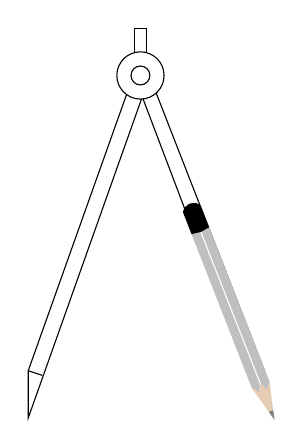
\begin{tikzpicture}
\begin{scope}[rotate=0,transform shape,scale=3]
\draw (2.95,3.7) rectangle (3,3.95);
\draw (2.92,3.68) -- (2.5,2.5) -- (2.5,2.3) -- (2.99,3.68);
\draw (3.5,2.5) -- (3.43,2.48) -- (2.975,3.68);
\draw (3.04,3.68) -- (3.5,2.5);
\draw (2.5,2.5) -- (2.56,2.48);
\draw[fill=white] (2.975,3.75) circle (0.1cm);
\draw (2.975,3.75) circle (0.04cm);
\end{scope}
\begin{scope}[xshift=10.34cm,yshift=7.28cm,rotate=21.4,scale=.6]          
\fill[gray!50] (0,4) -- (0.4,4) -- (0.4,0) --
               (0.3,-0.15) -- (0.2,0) -- (0.1,-0.14) --
               (0,0) -- cycle;
\draw[color=white] (0.2,4) -- (0.2,0);
\fill[black] (0,3.5) -- (0.2,3.47) -- (0.4,3.5) --
             (0.4,4) arc(30:150:0.23cm);
\fill[brown!40] (0,0) -- (0.2,-0.8)
    node[coordinate,pos=0.75](a){} -- 
    (0.4,0)node[coordinate,pos=0.25](b){} -- 
    (0.3,-0.15) -- (0.2,0) -- (0.1,-0.14) -- cycle;
\fill[gray] (a) -- (0.2,-0.8) -- (b) -- cycle;
\end{scope}
\end{tikzpicture}
}
\hspace{3em}
\subcaptionbox{%
מחוגה מתמוטטת. המשתמש מצמיד חוט למרכז המעגל. לקצה השני של החוט מחובר עפרון המשמש לשרטוט המעגל. כאשר מרימים את המחוגה מהנייר, האצבעות (מקווקווים) יכולים בקלות להחליק למקום אחר.%
\label{fig.collapsing-compass}}
[.45\textwidth]
{
\centering
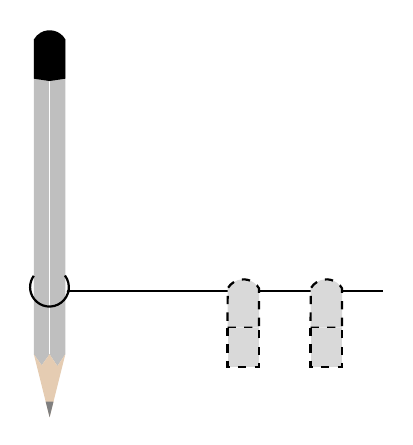
\begin{tikzpicture}[rotate=0,scale=1]          
\fill[gray!50] (0,4) -- (0.4,4) -- (0.4,0) --
               (0.3,-0.15) -- (0.2,0) -- (0.1,-0.14) --
               (0,0) -- cycle;
\draw[color=white] (0.2,4) -- (0.2,0);
\fill[black] (0,3.5) -- (0.2,3.47) -- (0.4,3.5) --
             (0.4,4) arc(30:150:0.23cm);
\fill[brown!40] (0,0) -- (0.2,-0.8)
    node[coordinate,pos=0.75](a){} -- 
    (0.4,0) node[coordinate,pos=0.25](b){} -- 
    (0.3,-0.15) -- (0.2,0) -- (0.1,-0.14) -- cycle;
\fill[gray] (a) -- (0.2,-0.8) -- (b) -- cycle;

\draw[thick] (0.395,1) arc (37:-216:7pt);
\coordinate (knot) at (0.44,.8);
\draw[thick] (knot) -- +(4,0);
\fill (knot) circle (.7pt);

\begin{scope}[xshift=100pt,yshift=-90pt]
\draw[dashed,thick,fill=white!70!gray] (0,3.5) -- (0.4,3.5) -- 
      (0.4,4) arc(30:150:0.23cm) -- cycle;
\draw[dashed,thick,fill=white!70!gray] (0,3.5) -- ++(0,-.5) -- ++(.4,0) -- ++(0,.5);
\end{scope}

\begin{scope}[xshift=70pt,yshift=-90pt]
\draw[dashed,thick,fill=white!70!gray] (0,3.5) -- (0.4,3.5) -- 
      (0.4,4) arc(30:150:0.23cm) -- cycle;
\draw[dashed,thick,fill=white!70!gray] (0,3.5) -- ++(0,-.5) -- ++(.4,0) -- ++(0,.5);
\end{scope}
\end{tikzpicture}
}
\end{figure}

בתחילת הפרק דיון על הרלוונטית של למידה של בניה עם סרגל ומחוגה (סעיף%
~\ref{s.relevance}).
סעיף%
~\ref{s.collapse} 
משווה את שני סוגי המחוגה בבניה הפשוטה ביותר: אנח אמצעי. סעיף%
~\ref{s.collapse-copy}
מביא את השיטה של אוקלידס להעתקת קטע קו באמצעות מחוגה מתמוטטת. זה מוכיח שניתן לבצע באמצעות מחוגה מתמוטטת כל בניה שניתנת לביצוע באמצעות מחוגה קבועה. סעיף%
~\ref{s.collapse-copy-incorrect} 
מציג הוכחה של משפט זה שנראית נכונה אבל שלא עובדת עבור כל תצורה של קווים ונקודות. כדי להדגיש שאין לסמוך על שרטוט, סעיף%
~\ref{s.collapse-isoceles}
מביא "הוכחה לכאורה" מפורסמת ש-
\textbf{כל}
משולש הוא שווי שוקיים. ההוכחה נראית נכונה אבל היא שגויה כי היא מתבססת על שרטוט לא נכון.

%%%%%%%%%%%%%%%%%%%%%%%%%%%%%%%%%%%%%%%%%%%%%%%%%%%%%%%%%%%%%%%

\section{בניה עם סרגל ומחוגה}\label{s.relevance}

%%%%%%%%%%%%%%%%%%%%%%%%%%%%%%%%%%%%%%%%%%%%%%%%%%%%%%%%%%%%%%%

\section{מחוגה קבועה ומחוגה מתמוטטת}\label{s.collapse}

$\overline{AB}$
שווה כמובן לאורך של
$\overline{BA}$,
ולכן למעגלים רדיוס זהה.

בבניה עם המחוגה המתמוטטת קל להוכיח שמתקבל משולש שווה-צלעות. האורך של
$\overline{AC}$
שווה לאורכו של
$\overline{AB}$,
כי שניהם רדיוסים של אותו מעגל, ומאותה סיבה האורך של
$\overline{BC}$
שווה לאורכו של
$\overline{BA}$.
מכאן ש-%
$\overline{AC} = \overline{AB} = \overline{BA} = \overline{BC}$.

הבניה של משולש שווה-צלעות היא המשפט הראשון בספר של אוקלידס. המשפט השני מראה שאפשר להעתיק קטע קו עם מחוגה מתמוטטת, ולכן המחוגה הקבועה לא מוסיפה יכולת חדשה. 

בספרי לימוד גיאומטריה ניתן למצוא בנייה של אנך אמצעי לקטע קו על ידי בניית שני מעגלים שמרכזם על הקו, 
\textbf{ובלבד שהרדיוס גדול ממחצית המרחק בין המרכזים},
)תרשים שמאלי(:

%%%%%%%%%%%%%%%%%%%%%%%%%%%%%%%%%%%%%%%%%%%%%%%%%%%%%%%%%%%%%%%


\section{העתקת קטע קו לפי אוקלידס}\label{s.collapse-copy}

\begin{theorem}
נתון קטע קו
$AB$
ונקודה
$C$
(איור%
~\ref{f.euclid},
משמאל), ניתן לבנות עם מחוגה מתמוטטת בנקודה
$C$
קטע קו שאורכו שווה לאורכו של 
$AB$.
\end{theorem}

\begin{figure}
\begin{center}
\begin{tikzpicture}[scale=0.6]
\begin{scope}
\coordinate (C) at (0,0);
\coordinate (A) at (2.5,0);
\coordinate (B) at (5.5,2);
\draw (A) node[below,xshift=-2pt,yshift=-2pt] {$A$} -- (B) node[right] {$B$};
\fill (A) circle[radius=3pt];
\fill (B) circle[radius=3pt];
\fill (C) node[below,xshift=2pt,yshift=-2pt] {$C$} circle[radius=3pt];
\end{scope}
\begin{scope}[xshift=12cm]
\coordinate (C) at (0,0);
\coordinate (A) at (2.5,0);
\coordinate (B) at (5.5,2);
\draw (A) node[below,xshift=-2pt,yshift=-2pt] {$A$} -- (B) node[right] {$B$};
\fill (A) circle[radius=3pt];
\fill (B) circle[radius=3pt];
\fill (C) node[below,xshift=2pt,yshift=-2pt] {$C$} circle[radius=3pt];
\draw (A) -- (C);
\path[name path=larc] (C) ++(-70:2.5cm) arc (-70:70:2.5cm);
\path[name path=rarc] (A) ++(-110:2.5cm) arc (-110:-250:2.5cm);
\path [name intersections={of=larc and rarc,by={d,D}}];
\fill (D) node[above] {$D$} circle[radius=3pt];
\draw (A) -- (D);
\draw (C) -- (D);
\end{scope}
\end{tikzpicture}
\end{center}
\caption{בנייה של אוקלידס}\label{f.euclid}
\end{figure}

\begin{proof}
\textbf{בניה:}
\begin{itemize}
\item
חברו בקו את הנקודות
$A$
ו-%
$C$.
\item
בנו משולש שווה צלעות שבסיסו
$\overline{AC}$
)אפשרי לפי המשפט הראשון של אוקלידס(.
סמנו את הקודקוד של המשולש ב-%
$D$
)תרשים ימני למעלה(. 
\item
בנו קרן בהמשך של
$\overline{DA}$
וקרן בהמשך של 
$DC$
)תרשים שמאלי למטה(.
\item
בנו מעגל שמרכזו 
$A$
עם רדיוס
$\overline{AB}$.
סמנו
$E$,
החיתוך של המעגל עם הקרן
$\overline{DE}$
)תרשים ימני(.

\begin{center}

\begin{tikzpicture}[scale=0.6]
\begin{scope}
\coordinate (C) at (0,0);
\coordinate (A) at (2.5,0);
\coordinate (B) at (5.5,2);
\draw (A) node[below,xshift=-2pt,yshift=-2pt] {$A$} -- (B) node[right] {$B$};
\fill (A) circle[radius=3pt];
\fill (B) circle[radius=3pt];
\fill (C) node[below,xshift=2pt,yshift=-2pt] {$C$} circle[radius=3pt];
\draw (A) -- (C);
\path[name path=larc] (C) ++(-70:2.5cm) arc (-70:70:2.5cm);
\path[name path=rarc] (A) ++(-110:2.5cm) arc (-110:-250:2.5cm);
\path [name intersections={of=larc and rarc,by={d,D}}];
\fill (D) node[above] {$D$} circle[radius=3pt];
\draw (A) -- (D);
\draw (C) -- (D);
\draw[name path=ray2] (D) -- ($ (D) ! 2.7 ! (C) $);
\draw[name path=ray1] (D) -- ($ (D) ! 2.7 ! (A) $);
\end{scope}
\begin{scope}[xshift=12cm]
\coordinate (C) at (0,0);
\coordinate (A) at (2.5,0);
\coordinate (B) at (5.5,2);
\draw (A) node[below,xshift=-2pt,yshift=-2pt] {$A$} -- (B) node[right] {$B$};
\fill (A) circle[radius=3pt];
\fill (B) circle[radius=3pt];
\fill (C) node[below,xshift=2pt,yshift=-2pt] {$C$} circle[radius=3pt];
\draw (A) -- (C);
\path[name path=larc] (C) ++(-70:2.5cm) arc (-70:70:2.5cm);
\path[name path=rarc] (A) ++(-110:2.5cm) arc (-110:-250:2.5cm);
\path [name intersections={of=larc and rarc,by={d,D}}];
\fill (D) node[above] {$D$} circle[radius=3pt];
\draw (A) -- (D);
\draw (C) -- (D);
\draw[name path=ray2] (D) -- ($ (D) ! 2.7 ! (C) $);
\draw[name path=ray1] (D) -- ($ (D) ! 2.7 ! (A) $);
\node[draw,circle through=(B),name path=c1] at (A) {};
\path [name intersections={of=c1 and ray1,by={E,e}}];
\fill (E) node[right,xshift=2pt,yshift=-2pt] {$E$} circle[radius=3pt];
\end{scope}
\end{tikzpicture}
\end{center}
\item
בנו מעגל שמרכזו 
$D$
עם רדיוס 
$\overline{DE}$.
סמנו את החיתוך של
$\overline{DC}$
עם המעגל ב-%
$F$:
\end{itemize}

\begin{center}

\begin{tikzpicture}[scale=0.4]
\coordinate (C) at (0,0);
\coordinate (A) at (2.5,0);
\coordinate (B) at (5.5,2);
\draw (A) node[below,xshift=-2pt,yshift=-2pt] {$A$} -- node[above] {$x$} (B) node[right] {$B$};
\fill (A) circle[radius=3pt];
\fill (B) circle[radius=3pt];
\fill (C) node[below,xshift=2pt,yshift=-2pt] {$C$} circle[radius=3pt];
\draw (A) -- (C);
\path[name path=larc] (C) ++(-70:2.5cm) arc (-70:70:2.5cm);
\path[name path=rarc] (A) ++(-110:2.5cm) arc (-110:-250:2.5cm);
\path [name intersections={of=larc and rarc,by={d,D}}];
\fill (D) node[above] {$D$} circle[radius=3pt];
\draw (A) -- node[right] {$y$} (D);
\draw (C) -- node[left] {$y$} (D);
\draw[name path=ray2] (D) -- ($ (D) ! 3 ! (C) $);
\draw[name path=ray1] (D) -- ($ (D) ! 3 ! (A) $);
\node[draw,circle through=(B),name path=c1] at (A) {};
\path [name intersections={of=c1 and ray1,by={E,e}}];
\fill (E) node[right,xshift=2pt,yshift=-2pt] {$E$} circle[radius=3pt];
\node[draw,circle through=(E),name path=c2] at (D) {};
\path [name intersections={of=c2 and ray2,by={F,f}}];
\fill (F) node[left,xshift=-2pt,yshift=-2pt] {$F$} circle[radius=3pt];
\path (A) -- node[right] {$x$} (E);
\path (C) -- node[left] {$x$} (F);
\end{tikzpicture}
\end{center}

\textbf{טענה:}
אורכו של קטע הקו
$\overline{CF}$
שווה לאורכו של קטע הקו
$\overline{AB}$.


\textbf{הוכחה:}
$\overline{DC}=\overline{DA}$
כי
$\triangle ACD$
שווה-צלעות.
$\overline{AE}=\overline{AB}$
כי שניהם רדיוסים של המעגל שמרכזו 
$A$.
$\overline{DF}=\overline{DE}$
כי שניהם רדיוסים של המעגל שמרכזו
$D$.
אורכו של
$\overline{CF}$ 
הוא:
\[
\overline{CF} = \overline{DF} - \overline{DC} = \overline{DE} - \overline{DC} = \overline{DE} - \overline{DA} = \overline{AE} = \overline{AB}\,.
\].
\end{proof}

%%%%%%%%%%%%%%%%%%%%%%%%%%%%%%%%%%%%%%%%%%%%%%%%%%%%%%%%%%%%%%%

\section{העתקה שגויה של קטע קו}\label{s.collapse-copy-incorrect}

\begin{itemize}
\item
בנו מעגל שמרכזו
$A$
עם רדיוס
$\overline{AB}$:
\begin{center}

\begin{tikzpicture}[scale=0.6]
\begin{scope}
\coordinate (C) at (-2,0);
\coordinate (A) at (2.5,0);
\coordinate (B) at (4.5,1.5);
\draw (A) node[below,xshift=-2pt,yshift=-2pt] {$A$} -- (B) node[right] {$B$};
\fill (A) circle[radius=3pt];
\fill (B) circle[radius=3pt];
\fill (C) node[below,xshift=2pt,yshift=-2pt] {$C$} circle[radius=3pt];
\end{scope}
\begin{scope}[xshift=12cm]
\coordinate (C) at (-2,0);
\coordinate (A) at (2.5,0);
\coordinate (B) at (4.5,1.5);
\draw (A) node[below,xshift=-2pt,yshift=-2pt] {$A$} -- (B) node[right] {$B$};
\fill (A) circle[radius=3pt];
\fill (B) circle[radius=3pt];
\fill (C) node[below,xshift=2pt,yshift=-2pt] {$C$} circle[radius=3pt];
\node[draw,circle through=(B),name path=c1] at (A) {};
\end{scope}
\end{tikzpicture}
\end{center}
%\vspace*{-8ex}
\item
בנו מעגל שמרכזו
$A$
עם רדיוס
$\overline{AC}$
ומעגל שמרכזו
$C$
עם רדיוס
$\overline{AC}=\overline{CA}$.
\item
סמנו את נקודות החיתוך של המעגלים ב-%
$E,F$.
סמנו את נקודת החיתוך של המעגל שמרכזו
$C$
עם המעגל שמרכזו 
$A$
עם רדיוס
$\overline{AB}$
ב-%
$D$:
\begin{center}

\begin{tikzpicture}[scale=0.6]
\coordinate (C) at (-2,0);
\coordinate (A) at (2.5,0);
\coordinate (B) at (4.5,1.5);
\draw (A) node[below right] {$A$} -- (B) node[right] {$B$};
\fill (A) circle[radius=3pt];
\fill (B) circle[radius=3pt];
\fill (C) node[left,xshift=-2pt] {$C$} circle[radius=3pt];
\node[draw,circle through=(B),name path=c1] at (A) {};
\node[draw,circle through=(C),name path=c2] at (A) {};
\node[draw,circle through=(A),name path=c3] at (C) {};
\path [name intersections={of=c1 and c3,by={D,f}}];
\path [name intersections={of=c2 and c3,by={E,F}}];
\fill (D) node[below right,xshift=4pt] {$D$} circle[radius=3pt];
\fill (E) node[above,yshift=2pt] {$E$} circle[radius=3pt];
\fill (F) node[below,yshift=-2pt] {$F$} circle[radius=3pt];
\end{tikzpicture}
\end{center}
\item
בנו מעגל שמרכזו 
$E$
עם רדיוס 
$\overline{ED}$.
סמנו ב-%
$G$
את החיתוך של המעגל עם המעגל שמרכזו
$A$
עם רדיוס 
$\overline{AC}$
)איור~%
\ref{f.collapse1}(.
\end{itemize}
\begin{figure}[tb]
\begin{center}

\begin{tikzpicture}[scale=0.8]
\clip (-8,-1) rectangle (9,5);
\coordinate (C) at (-2,0);
\coordinate (A) at (2.5,0);
\coordinate (B) at (4.5,1.5);
\draw[thick] (A) node[below right] {$A$} -- (B) node[right] {$B$};
\fill (A) circle[radius=3pt];
\fill (B) circle[radius=3pt];
\fill (C) node[below left] {$C$} circle[radius=3pt];
\node[draw,circle through=(B),name path=c1] at (A) {};
\node[draw,circle through=(C),name path=c2] at (A) {};
\node[draw,circle through=(A),name path=c3] at (C) {};
\path [name intersections={of=c1 and c3,by={D,f}}];
\path [name intersections={of=c2 and c3,by={E,F}}];
\fill (D) node[below right,xshift=4pt] {$D$} circle[radius=3pt];
\fill (E) node[above,yshift=2pt] {$E$} circle[radius=3pt];
\fill (F) node[below,yshift=-2pt] {$F$} circle[radius=3pt];
\node[draw,circle through=(D),name path=c4] at (E) {};
\path [name intersections={of=c2 and c4,by={g,G}}];
\fill (G) node[below left,xshift=-4pt] {$G$} circle[radius=3pt];
\draw[thick] (C) -- (G);
\draw[thick,dashed] (G) -- (E) -- (C);
\draw[thick,dashed] (A) -- (D) -- (E) -- cycle;
\end{tikzpicture}
\end{center}
\selectlanguage{hebrew}
\caption{משולשים חופפים}\label{f.collapse1}
\end{figure}

\textbf{טענה:}
ארכו של 
$\overline{CG}$
שווה לאורכו של
$\overline{AB}$.

\textbf{הוכחה:}
נניח ש-%
$\triangle ADE\cong \triangle CGE$.
אם כן, 
$\overline{CG}=\overline{AD}=\overline{AB}$
כי 
$\overline{AD},\overline{AB}$
הם רדיוסים של המעגל הקטן שמרכזו 
$A$.
למעגל שמרכזו
$C$
אותו רדיוס כמו למעגל שמרכזו 
$A$
ועובר דרך 
$E$.
לכן, ניתן להתייחס אליהם כ-"אותו" מעגל.

עכשיו נוכיח את החפיפה
$\triangle ADE\cong \triangle CGE$.
$\overline{EG}=\overline{ED}$
כי הם רדיוסים של המעגל שמרכזו
$E$,
ו-%
$\overline{EC}=\overline{EA}$
כי הם רדיוסים של "אותו" מעגל. 
$\angle GCE=\angle DAE$
כי הן זוויות היקפיות על "אותו" מיתר 
$\overline{EG},\overline{ED}$.
 $\angle CGE=\angle ADE$
כי הן זוויות היקפיות על "אותו" מיתר
$\overline{EC},\overline{EA}$.
. לכן,
$\angle GEC=\angle DEA$
ו-%
$\triangle ADE\cong \triangle CGE$
לפי צ.ז.צ.
\qed

אין שום שגיאה בהוכחה! השגיאה נובעת ממקור אחר: השווין
$\overline{AB}=\overline{GC}$
מתקיים רק כאשר אורכו של 
$\overline{AB}$
קטן מאורכו של
$\overline{AC}$.
הבנייה של אוקלידס נכונה ללא קשר לאורך היחסי של הקווים ולמיקום של הנקודה
$C$
ביחס לקטע הקו
$\overline{AB}$.

%%%%%%%%%%%%%%%%%%%%%%%%%%%%%%%%%%%%%%%%%%%%%%%%%%%%%%%%%%%%%%%

\section{
אין לסמוך על תרשים
}\label{s.collapse-isoceles}
בסעיף~%
\ref{s.collapse-copy-incorrect}
ראינו שאין לסמוך על ציור. הנה הוכחה "נכונה"
\textbf{\R{שכל}}
משולש שווה-שוקיים!

\begin{figure}[tb]
\begin{center}

\begin{tikzpicture}[scale=1.2]
\coordinate (P) at (0,0);
\node[xshift=4mm,yshift=1mm] at (P) {$P$};
\coordinate [label=left:$B$] (B)  at (-2,-2);
\coordinate [label=right:$C$] (C)  at (4,-2);
\coordinate [label=above:$A$] (A)  at (-1,2);
\node[below,yshift=-12pt,xshift=2pt] at (A) {$\alpha$};
\node[below,yshift=-12pt,xshift=15pt] at (A) {$\alpha$};
\draw (A) -- (B);
\draw (A) -- (C);
\draw (B) -- (C);
\draw (A) -- (P);
\draw (B) -- (P);
\draw (C) -- (P);
\coordinate[label=left:$E$] (E) at ($ (A) ! .44 ! (B) $);
\draw[rotate=-100] (E) rectangle +(8pt,8pt);
\draw (P) -- (E);
\coordinate[label=right:$F$] (F) at ($ (A) ! .33 ! (C) $);
\draw[rotate=-132] (F) rectangle +(8pt,8pt);
\draw (P) -- (F);
\coordinate[label=below:$D$] (D) at ($ (B) ! .33 ! (C) $);
\draw (D) rectangle +(8pt,8pt);
\draw (P) -- (D);
\node[left] at ($ (A) ! .5 ! (E) $) {};
\node[left] at ($ (B) ! .5 ! (E) $) {};
\node[below] at ($ (B) ! .5 ! (D) $) {$a$};
\node[below] at ($ (C) ! .5 ! (D) $) {$a$};
\node[right,xshift=2pt] at ($ (A) ! .5 ! (F) $) {};
\node[right,xshift=2pt] at ($ (C) ! .5 ! (F) $) {};
%\fill (A) circle(1pt);
%\fill (B) circle(1pt);
%\fill (C) circle(1pt);
\fill (D) circle(1pt);
\fill (E) circle(1pt);
\fill (F) circle(1pt);
\fill (P) circle(1pt);
\end{tikzpicture}
\end{center}
\selectlanguage{hebrew}
\caption{"הוכחה" שכל משולש שווה-שוקיים}\label{f.isoceles}
\end{figure}

נתון משולש שרירותי 
$\triangle ABC$,
תהי
$P$
נקודת החיתוך בין חוצה הזווית של
$\angle BAC$
לבין האנך האמצעי של 
$\overline{BC}$
)איור
\ref{f.isoceles}(.
סמנו ב-%
$D,E,F$
את נקודות החיתוך של האנכים מ-%
$P$
לצלעות
$\overline{BC},\overline{AB},\overline{AC}$. $\triangle APE\cong \triangle APF$
כי הם משולשים ישר זווית עם זוויות שוות
$\alpha$
וצלע 
$\overline{AP}$
משותף.

$\triangle DPB\cong \triangle DPC$
לפי צ.ז.צ. כי 
$\overline{PD}$
הוא צלע משותף, 
$\angle PDB=\angle PDC=90^\circ$,
ו-%
$\overline{BD}=\overline{DC}=a$
כי 
$\overline{PD}$
הוא האנך האמצעי ל-%
$\overline{BC}$.
במשולשים ישר-זווית
$\triangle EPB\cong \triangle FPC$
כי שתי לצועות שוות:
$\overline{EP}=\overline{PF}$
לפי החפיפה הראשונה, ו-%
$\overline{PB}=\overline{PC}$
לפי החפיפה השנייה. נחבר את השוויונות ונקבל ש-%
$\triangle ABC$
שווה-שוקיים:
\[
\overline{AB}=\overline{AE}+\overline{EB}=\overline{AF}+\overline{FC}=\overline{AC}\,.
\]
\qed
הבעיה בהוכחה היא שתרשים אינו נכון כי הנקודה
$P$
נמצאת
\textbf{מחוץ}
למשולש כפי שניתן לראות מהציור המדוייק באיור%
~\ref{f.isoceles-wrong}.
\begin{figure}
\begin{center}

\begin{tikzpicture}[scale=.9]
\coordinate (B)  at (0,0);
\node[left] at (B) {$B$};
\coordinate (C)  at (7,0);
\node[right] at (C) {$C$};
\path[name path=pathb] (B) -- +(80:6.5);
\path[name path=pathc] (C) -- +(140:9.5);
\path [name intersections={of=pathb and pathc,by={A}}];
\node[above] at (A) {$A$};
%\fill (A) circle(1pt) node[above] {$A$};
%\fill (B) circle(1pt) node[left] {$B$};
%\fill (C) circle(1pt) node[right] {$C$};
\draw (A) -- (B) -- (C) -- cycle;
\draw[name path=angle] (A) -- +(-70:8.5);
\draw ($(B)!.5!(C)$) |- +(0,4);
\draw[name path=perp] ($(B)!.5!(C)$) |- +(0,-3);
\draw ($(B)!.5!(C)$) rectangle +(8pt,8pt);
\path [name intersections={of=angle and perp,by={P}}];
\fill (P) circle(3pt) node[right] {$P$};
\node[below,yshift=-12pt,xshift=2pt] at (A) {$\alpha$};
\node[below,yshift=-12pt,xshift=15pt] at (A) {$\alpha$};
\end{tikzpicture}
\end{center}
\caption{נקודת החיתוך בין חוצה הזווית והאנך האמצעי}\label{f.isoceles-wrong}
\end{figure}

\selectlanguage{hebrew}


\subsection*{מקורות}

\L{Toussaint} \L{\cite{toussaint}}
הראה שפורסמו הוכחות שגויות רבות של המשפט ודווקא אוקלידס הוא זה שנתן הוכחה נכונה! הבניה בסעיף~%
\ref{s.collapse-copy-incorrect}
לקוחה מ-%
\L{\cite{rusty}}
ו-%
\L{\cite{toussaint}}.
